% Frugal AI seminar, project 2: a LangGraph workflow on your own notes (FrugalAI/code/workflow-agent, faqintake).
% Procedure and theory only, no results. CheatSheet-safe: no floats, the table is wrapped in adjustbox.

\section[Notes Flow]{Project: A Workflow on Your Own Notes}

%%%%%%%%%%%%%%%%%%%%%%%%%%%%%%%%%%%%%%%%%%%%%%%%%%%
\begin{frame}[fragile]\frametitle{}
\begin{center}
{\Large Project: A Workflow on Your Own Notes}

\medskip
{\small (A LangGraph graph built from a procedure you already follow)}
\end{center}
\end{frame}

%%%%%%%%%%%%%%%%%%%%%%%%%%%%%%%%%%%%%%%%%%%%%%%%%%%
\begin{frame}[fragile]\frametitle{Theory: Turn a Written Procedure Into a Graph}
\begin{itemize}
\item A workflow is a graph of steps with shared state. Edges can fan out in parallel, join, branch on a condition, and loop.
\item Start from a procedure that already exists. Split every step by who should do it: code, a small model, or a person.
\item Rule of thumb: code for counting, searching, routing, checking and planning; the model for wording; a person for facts and judgment.
\end{itemize}
\begin{center}
\scriptsize
\adjustbox{max width=\linewidth}{%
\begin{tabular}{p{0.36\linewidth}p{0.56\linewidth}}
\hline
Procedure step & Who does it \\
\hline
Check what already exists & Code: a regex counter, plus embedding search \\
Plan, then confirm & Code writes the plan; a person confirms \\
Write an entry from notes & Model fills a few fields; code adds the skeleton \\
Verify facts, write chapters & A person or a stronger model, outside the graph \\
Propagate to other files & Code lists them in order; nothing is edited \\
\hline
\end{tabular}}
\end{center}
{\tiny (Ref: LangGraph; FrugalAI code/workflow-agent, faqintake)}
\end{frame}

%%%%%%%%%%%%%%%%%%%%%%%%%%%%%%%%%%%%%%%%%%%%%%%%%%%
\begin{frame}[fragile]\frametitle{Procedure: Parallel Checks, a Router, a Repair Loop}
\begin{center}
\adjustbox{max width=0.97\linewidth, max totalheight=0.3\textheight}{%
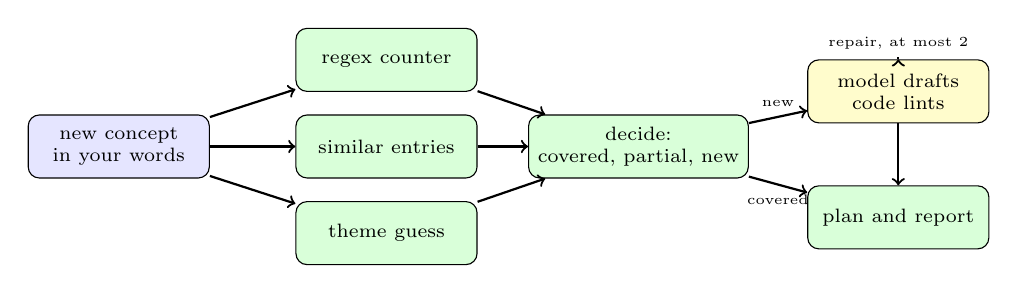
\begin{tikzpicture}
\tikzstyle{b}=[draw, rounded corners, align=center, minimum height=0.8cm, minimum width=2.3cm, font=\scriptsize]
\node[b, fill=blue!10] (i) at (0,0) {new concept\\in your words};
\node[b, fill=green!15] (a) at (3.4,1.1) {regex counter};
\node[b, fill=green!15] (s) at (3.4,0) {similar entries};
\node[b, fill=green!15] (t) at (3.4,-1.1) {theme guess};
\node[b, fill=green!15] (d) at (6.6,0) {decide:\\covered, partial, new};
\node[b, fill=yellow!20] (w) at (9.9,0.7) {model drafts\\code lints};
\node[b, fill=green!15] (p) at (9.9,-0.9) {plan and report};
\draw[->, thick] (i) -- (a);
\draw[->, thick] (i) -- (s);
\draw[->, thick] (i) -- (t);
\draw[->, thick] (a) -- (d);
\draw[->, thick] (s) -- (d);
\draw[->, thick] (t) -- (d);
\draw[->, thick] (d) -- node[above, font=\tiny] {new} (w);
\draw[->, thick] (d) -- node[below, font=\tiny] {covered} (p);
\draw[->, thick] (w) -- (p);
\draw[->, thick] (w.north) to[out=60,in=120,looseness=6] node[above, font=\tiny] {repair, at most 2} (w.north);
\end{tikzpicture}}
\end{center}
\begin{itemize}
\item Three checks run in parallel and join at one decision node. A new concept enters a drafting sub-graph with a lint and repair loop.
\item State is a typed dictionary; a reducer merges each node's trace into one list.
\end{itemize}
{\tiny (Ref: LangGraph state graphs, conditional edges, sub-graphs)}
\end{frame}

%%%%%%%%%%%%%%%%%%%%%%%%%%%%%%%%%%%%%%%%%%%%%%%%%%%
\begin{frame}[fragile]\frametitle{Implementation: Detect, Draft, Lint}
\begin{itemize}
\item Duplicate check: embed each existing entry's title and question once. Embed the new concept and take the cosine similarity of the nearest entries. One threshold, calibrated on half of a labelled set and tested on the other half, splits covered from new. A band below it means ``needs review''.
\item The author's own regex counter is loaded and reused, not copied, so the graph and the procedure cannot drift apart.
\item Draft: the model returns a few fields as structured JSON (a schema, with a regex fallback). Code adds the headings, the sources section and a closing line that always says ``unverified draft''.
\item Lint: the house format as code, tested against every real entry. A dash fixer and a topic-drift check (the draft must use the notes' words) feed the repair loop.
\item Evaluate by leaving one real entry out, giving the model only its answer as notes, and comparing the draft with the real entry and with a one-prompt baseline.
\end{itemize}
{\tiny (Ref: FrugalAI code/workflow-agent; nothing is ever written into the knowledge base)}
\end{frame}

%%%%%%%%%%%%%%%%%%%%%%%%%%%%%%%%%%%%%%%%%%%%%%%%%%%
\begin{frame}[fragile]\frametitle{Design Rules and Pitfalls}
\begin{itemize}
\item Never let the workflow write into the real knowledge base. It writes a draft and a report; a person moves it.
\item Mark every machine draft as unverified, in code, not in the prompt.
\item Skip backup folders when indexing, or every concept will look ``covered''.
\item Pitfall: a small model shown a nearby example tends to copy its subject, not only its style. Show style with an unrelated example, and add a check that the draft uses the notes' words.
\item Run parallel branches for clarity, not speed: one local server mostly serves them one after another.
\end{itemize}
{\tiny (Ref: FrugalAI code/workflow-agent README)}
\end{frame}
